\documentclass[a4paper]{report}
% Use swiss german letters
\usepackage[utf8]{inputenc}
% Language: english
\usepackage[english]{babel}
% Fancy Figures
\usepackage{graphicx}
% Use Times
\usepackage{mathptmx}
% Display the Bibliography in the TOC
\usepackage{tocbibind}
% Better lists
\usepackage{enumitem}
% Shaded Boxes
\usepackage[svgnames]{xcolor}
\usepackage{framed}
\usepackage{mdframed}
% Use biblatex
\usepackage[style=apa,backend=biber,citestyle=authoryear]{biblatex} 
% Define the bibliography file
\addbibresource{bibliography.bib}
% To let LaTeX handle "
\usepackage[autostyle, english = british]{csquotes}
\DeclareLanguageMapping{english}{english-apa}
% To have text wrap around pictures
\usepackage{wrapfig}
% Define Shaded box
\definecolor{grey}{HTML}{C5C5C5}
\definecolor{lightgrey}{HTML}{E6E6E6}
\definecolor{lightblue}{HTML}{F0F7FD}
\definecolor{greyblue}{HTML}{D0E3F0}
\definecolor{darkblue}{HTML}{3A87AD}
\newmdenv[topline=false,rightline=false,bottomline=false,linecolor=greyblue,linewidth=2pt,backgroundcolor=lightblue]{quotebox}
% Blindtext package
% TODO remove
\usepackage{blindtext}

% Titlepage
\newcommand*{\titleAP}{\begingroup % Create the command for including the title page in the document
	\centering
	\vspace*{\baselineskip} % Whitespace at the top of the page
	
	{\Large Thushjandan Ponnudurai} and {\Large Pascal Baumann}\\[0.167\textheight] % Author name
	
	{\Huge\bfseries End-to-End Encryption mit IPv6 und integriertem IPSec}\\[\baselineskip]
	
	%TODO review subtitle
	{\Large \textit{Term paper NS FS2017}}\\
	\today
	
	\vspace*{3\baselineskip} % Whitespace at the bottom of the page
	\endgroup}

\graphicspath{{./img/}}

\begin{document}

\titleAP

\newpage

\begin{abstract}
	%TODO write abstract
	\blindtext
\end{abstract}

\tableofcontents

\newpage

\chapter{Theoretical part}
\label{ch:Theory}

\section{IP protocols}
\label{sec:IPprot}
The Internet Protocol (IP) is a set of rules governing how packets are transmitted over the internet. IP is probably the common protocol over the internet and is one of the layer 3 protocols (network layer) in the OSI model. It implements two basic functions:
\begin{itemize}
	\item Addressing hosts
	\item Routing datagrams (packets) from a source host to a destination host over multiple IP networks
\end{itemize}
A datagram is composed of an IP header and a payload. Source and destination IP addresses and other meta data are parts of the IP header and are needed to deliver a datagram. The payload includes the data that is transported.

IPv4 is the first major version and is at the moment the dominant protocol version of the internet. Due to a lack of IPv4 addresses the successor IPv6 was born. \parencite{NadeemUnuth2016}

\subsection{IPv4}
\label{ssec:IPv4}
Internet Protocol version 4 (IPv4) is specified in the IETF RFC 791 document and is existing since 1980. To route a packet across the networks, every host in the network has a logical address, which is the IPv4 address. This IPv4 addressing system is based on a 32-bit logical address, which amounts to 4'294'967'296 unique addresses.

An example of an IPv4 address is "148.21.45.110". The address is written in dot decimal notation and it has four octets of 8-bits. The binary form of this address will be 10010100.00010101.00101101.01101110. \parencite{Babatunde2014}

At the moment there is an IPv4 address exhaustion problem. Since the 3th of February 2011 Internet Corporation for Assigned Names and Numbers (ICANN) doesn't have any free blocks of IPv4 addresses. Due this problem IPv6 was developed and everything will be migrated in IPv6 over the long-term. 
\subsection{IPv6}
\label{ssec:IPv6}
Internet Protocol version 6 (IPv6) is the successor of IPv4. It was specified in 1998. The growth of the internet led to a need for a new alternative for IPv4. The problem is that IPv4 cannot provide the needed number of logical addresses around the world. For that reason IPv6 protocol was developed.\parencite[11]{Babatunde2014}

Several important areas were enhanced in the IPv6 protocol:
\begin{itemize}
	\item Expanded addressing
	\item Simplified header format
	\item Improved extension and option support
\end{itemize}
With the expanded address space the issue with the lack of addresses will be eliminated. Also the addressing architecture and the simplified header format helps improve the routing efficiency. Fewer packets needs to be processed thanks to the simplified header format. 
Every IPv6 packet has a fixed header length of 40 octets. But any options can be appended in extension headers after the IPv6 header. \parencite[106-107,123-124]{Loshin2004}

\subsubsection{IPv6 Addressing}
\label{sssec:ipv6:addressing}
There are three types of IPv6 addresses:
\begin{itemize}
	\item Unicast. A packet sent to an unicast address is delivered to the interface identified by that address.
	\item Multicast. A packet sent to a multicast address is delivered to all interfaces identified by that address. This address could be existing on different hosts.
	\item Anycast. A packet sent to a anycast address is delivered to one of the interfaces identified by that address. This address could be existing on different hosts.
\end{itemize}
Broadcast is not existing anymore in IPv6. \parencite[142-143]{Loshin2004}

The lenght of an IPv6 address is 128-bit. It is usually represented as 8 groups of up to 4 hexadecimal digits that are separated with colons. Each group stands for 16 bit.
\begin{quotebox}
	XXXX:XXXX:XXXX:XXXX:XXXX:XXXX:XXXX:XXXX
\end{quotebox}
Here is an example of an IPv6 address.
\begin{quotebox}
	2001:db8:1234:ABCD::10
\end{quotebox}
IPv6 addresses are usually divided into two equal 64-bit parts. The first 64-bit part identifies a network address and the last 64-bit part identifies the host.\parencite[144-146]{Loshin2004}
 
\subsubsection{IPv6 Headers}
\label{sssec:ipv6:headers}
The length of an header in IPv6 is not variable like in IPv4. It has a fixed length of 40 bytes. An IPv4 header can be as short as 20 bytes and as long as 60 bytes due to the IP options. Due to fixed header length in IPv6 packet handling is more efficient. Routers process usually always the options in the IPv4 header. Even if the options aren't relevant for the processing router. This leads to a degradation of the forwarding performance.  \parencite[128]{Loshin2004}

In the figure \ref{fig:IPv4_IPv6_Header} the IPv6 and IPv4 header are presented. It shows that an IPv6 header is simpler that an IPv4 header. The reason is that many attributes were removed in IPv6.
\begin{figure}
	\centering
	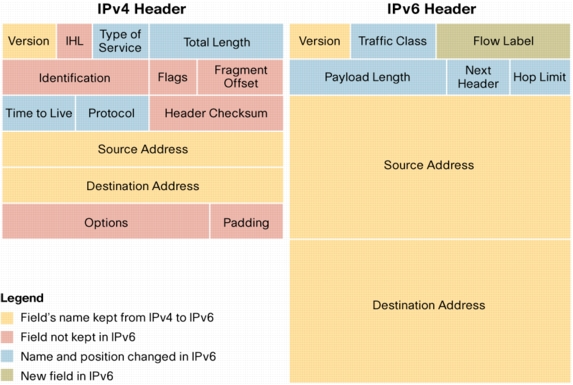
\includegraphics[width=0.8\linewidth]{ipv6_ipv4_headers}% no need to specify the file extension
	\caption {IPv4 and IPv6 Headers \cite{cisco2006}}
	\label{fig:IPv4_IPv6_Header}
\end{figure}

The IP option field is very important for the IP protocol operation. The functionality of IP options were removed from the main header and implemented in the extension headers. extension headers are a set of additional headers, which can be added as needed. So the routers will only process the main header and will process the extension headers only if it is required.

The figure~\ref{fig:IPv4_IPv6_ext_Header} explains how the extension headers are linked together in an IPv6 packet.
\begin{figure}
	\centering
	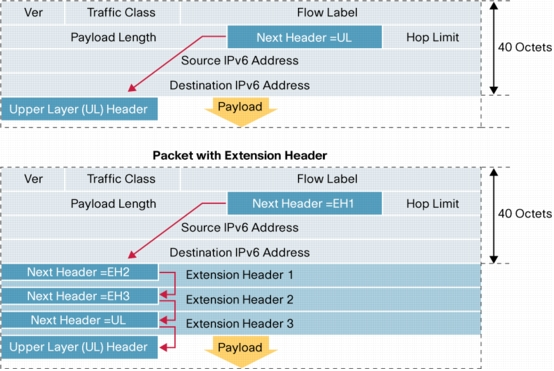
\includegraphics[width=0.8\linewidth]{ipv6_ipv4_ext_headers}% no need to specify the file extension
	\caption {IPv4 and IPv6 Headers \cite{cisco2006}}
	\label{fig:IPv4_IPv6_ext_Header}
\end{figure}
The extension headers are defined in RFC 2460 and their are shown in the table~\ref{tab:extension_header_codes} along with the Next Header values assigned to them. The recommended order, how the headers should be chained in a packet, is also defined in this RFC. \parencite[1-3]{cisco2006}
\begin{table}[]
	\centering
	\caption{Extension Headers and their recommended order in a packet}
	\label{tab:extension_header_codes}
	\begin{tabular}{lllll}
		\hline
		\textbf{Order}&  \textbf{Header Type}&  \textbf{Next Header Code}\\
		\hline
		1&  Basic IPv6 Header&  - \\
		2&  Hop-by-Hop Options
		Destination&  0 \\
		3&  Destination Options (with Routing Options)&  60 \\
		4&  Routing Header&  43 \\
		5&  Fragment Header&  44 \\
		6&  Authentication Header&  51 \\
		7&  Encapsulation Security Payload Header&  50 \\
		8&  Destination Options&  60 \\
		9&  Mobility Header&  135 \\
		&  No next header&  59 \\
		Upper layer&  TCP&  6 \\
		Upper layer&  UDP&  17 \\
		Upper layer&  ICMPv6&  58 \\
	\end{tabular}
\end{table}



\section{VPN protocol suites}
\label{sec:VPNs}

\subsection{SSL VPN}
\label{ssec:sslvpn}

\subsection{L2TP/PPTP}
\label{ssec:l2tppptp}

\subsection{IPSec}
\label{ssec:IPSec}


\chapter{Practical part}
\label{ch:Practical}

\newpage

\printbibliography

\end{document}          
